\documentclass{article}
\usepackage[utf8]{inputenc}
\usepackage{geometry}
\usepackage{graphicx}
\usepackage{float}
\geometry{legalpaper, portrait, margin=1.5in}
\usepackage{amsmath}
\title{%
	A Markowitz Portfolio Optimiser \\
	\large Computational Finance with C++ \\}
\author{CID: 01805027}
\date{10 June 2020}
\usepackage[thinc]{esdiff}
\usepackage{hyperref}
\usepackage{algorithm} 
\usepackage{algpseudocode} 
\usepackage{listings}
\usepackage{color}

\definecolor{dkgreen}{rgb}{0,0.6,0}
\definecolor{gray}{rgb}{0.5,0.5,0.5}
\definecolor{mauve}{rgb}{0.58,0,0.82}

\lstset{frame=tb,
	language=C++,
	aboveskip=3mm,
	belowskip=3mm,
	showstringspaces=false,
	columns=flexible,
	basicstyle={\small\ttfamily},
	numbers=none,
	numberstyle=\tiny\color{gray},
	keywordstyle=\color{blue},
	commentstyle=\color{dkgreen},
	stringstyle=\color{mauve},
	breaklines=true,
	breakatwhitespace=true,
	tabsize=3
}


\begin{document}
	
%\tableofcontents
	
	
\renewcommand*{\arraystretch}{1.5}

\maketitle
\section{Introduction} 
\label{sec:introduction}

Since their inception, economists, mathematicians, physicists and computer scientists the like have sought to 'beat' the markets using developments in their respective fields.

One such forum in which attempts have been made is the problem of portfolio choice. It is widely accepted that one of the goals of investing in financial markets is to make as much excess return as possible (above the standard market return; often characterised by the risk free rate) for a given level of risk taken on (idiosyncratic and non-idiosyncratic). 

This is characterised well by the \textit{Efficient Frontier} as seen in Figure (\ref{efficient_frontier}).


\begin{figure}[H]
	\centerline{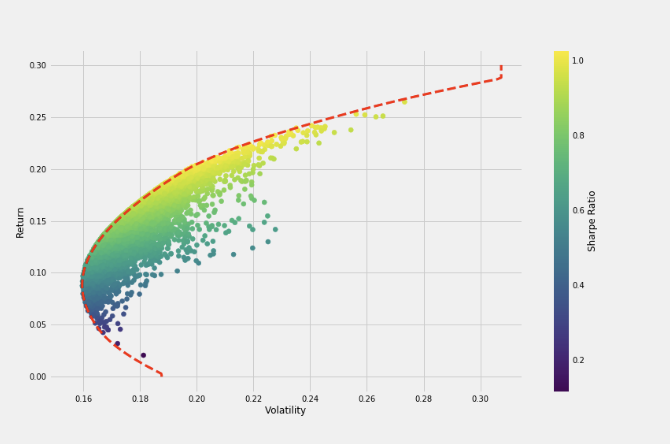
\includegraphics[width=\textwidth,height=4in]{figures/EF.png}}
	\label{efficient_frontier}
	\caption{Expected return against volatility. The red dashed line characterises the efficient frontier itself, on which the optimal portfolios lie. \cite{ef_medium} Note here the term \textit{volatility} is used to represent the variance of the portfolios, not the standard deviation as is traditional.}
\end{figure}


Optimal portfolios lie on the dashed red line, named the \textit{Efficient Frontier} as it characterises the portfolios that make as much excess return as possible for a given risk appetite, denoted by its position along the horizontal axis. The points in the centre of the concave function are examples of suboptimal portfolios. These portfolios carry more risk than the theory requires for their level of expected excess return, or similarly do not return enough above the market rate, for the amount of risk they take on.

No portfolios exist outside of the frontier since this scope corresponds to portfolios that achieve a theoretically impossibly large return for a given risk appetite, or conversely  and impossibly small level of risk for a quoted level of remuneration.


It must be noted that mean-variance efficiency is a corner-stone of modern portfolio choice theory, even appearing as an assumption to the renowned Capital Asset Pricing Model \cite{capm} (CAPM); it is assumed that 'all market participants are mean-variance efficient optimisers'. Though the subtle but important point must be made that the CAPM states that all market participants are rewarded for the amount of \textit{non-diversifiable, systematic risk} taken on, and says there shall be no remuneration for \textit{diversifiable, idiosyncratic risk} which are generally included in the measures of portfolio volatility used for the efficient frontier plot above.


As a result, this project seeks to solve the portfolio choice problem by an implementation of Markowitz Portfolio Theory \cite{mpt} in C++ using numerical methods and a backtesting framework to test the resulting portfolio.



\subsection{Theory}
\label{sec:theory}

The formal mathematical derivation below largely following notes provided by Parpas, P \cite{notes} are included for the context of the problem.

We define a target return, $\overline{r_p}$, for the portfolio and we wish for the portfolio to return this level of compensation for as little risk (portfolio variance) as possible. 

Therefore a system of Lagrange Multipliers are used to define the requirements on the portfolio. Namely, to:


\begin{enumerate}
	\item \textbf{Minimise portfolio variance, $\sigma_p^2$}  - Equation (\ref{portfolio_variance})

	\item \textbf{Ensure the expected portfolio return is equal to the target return, $\overline{r_p}$} - Equation (\ref{target_return_constraint})
	
	\item \textbf{Constrain the allocation of funds} - to ensure that the portfolio does not see an over or under-allocation of the funds available to it; it must have invested all resources available to it at any one time - Equation (\ref{weights_constraint})
	
\end{enumerate}

Note that there have been no constraints placed on the individual values of the portfolio weight of asset $i$, $w_i$. In other similar studies constraints such as ensuring the positivity of $w_i$ are employed to forbid the system from short selling a security. This constraint has not been imposed here; the model is freely able to short sell a security should it see fit.

In Equation (\ref{portfolio_variance}), we define the variance of the Markowitz portfolio, $\sigma_{p}^{2}$, with a preceding factor of $\frac{1}{2}$ for convenience. $\sigma_{ij}$ is the covariance between stocks $i$ and $j$.

DO WE WANNA ADD THE DERIVATION?

\begin{equation}
\dfrac{1}{2} \sigma^{2}_{p} =  \dfrac{1}{2} \sum_{i,j=1}^{n} w_{i} \sigma_{ij} w_{j}
\label{portfolio_variance}
\end{equation}

The variance of the portfolio is minimised via the Lagrange method while ensuring the following two constraints are also upheld:

\begin{equation}
\sum_{i=1}^{n} w_{i} \overline{r_i} - \overline{r_p} = 0
\label{target_return_constraint}
\end{equation}

Above, we mandate that the portfolio return is equal to the value target return $\overline{r_p}$. By setting $\overline{r_p}$, we have effectively chosen the portfolio return we desire and thus the weights the optimisation method yields.

Below, is simply the constraint that the sum of the portfolio weights must be equal to unity. This ensures that the portfolio does not over or under-allocate the funds available to it.

\begin{equation} 
\sum_{i=1}^{n} w_{i} - 1 = 0
\label{weights_constraint}
\end{equation}

\begin{equation} 
L(w, \lambda, \mu) =  \dfrac{1}{2} \sum_{i,j=1}^{n} w_{i} \sigma_{ij} w_{j} 
	-\lambda \left( \sum_{i=1}^{n} w_{i} \overline{r_i} - \overline{r_p}) \right)
	- \mu \left( \sum_{i=1}^{n} w_{i} - 1 \right)
\label{lagrangian}
\end{equation}

Finally, Equation(\ref{lagrangian}) shows the Lagrangian we seek to minimise, with $\lambda$ and $\mu$ the lagrange multipliers for points 

For convenience when scaling to a large number of assets and to code in the possibility of introducing further constraints, we introduce the following matrix notation:

\begin{description}
\item [$\bullet$ $\emph{w} = (w_1,..., w_n)' \in \Re^n$ ] - a column vector of $n$ weights for $n$ assets
\item [$\bullet$ $\overline{\emph{r}} = (\overline{r_1},..., \overline{r_n})' \in \Re^n$ ] - a column vector of $n$ expected asset returns
\item [$\bullet$ $\emph{e} = (1,..., 1)' \in \Re^n$ ] - the unit column vector of length $n$
\item [$\bullet$ $\emph{0} = (0,..., 0)' \in \Re^n$ ] - the zero column vector of length $n$
\end{description}

The Lagrangian in matrix form is shown below in Equation (\ref{vector_lagrangrian}) where $\Sigma \in \Re^{n \times n}$ is the covariance matrix of the assets, explicitly; $\Sigma_{ij} = \sigma_{ij}$ as defined above.

\begin{equation} 
L(\textbf{w}, \lambda, \mu)  = \dfrac{1}{2} \textbf{w}'\Sigma\textbf{w}
-\lambda \left( \textbf{w}'\overline{\textbf{r}} - \overline{r_p}\right)
-\mu \left( \textbf{w}'\textbf{e} - 1\right)
\label{vector_lagrangrian}
\end{equation}

Now, in order to minimise the Lagrangian it must be differentiated with respect to the weights, {\textbf{w}}. Allowing us to find the rate of change of the system's Lagrangian with respect to the portfolio weights and setting the resulting equation to zero will yeild the turning point of the function in parameter space.

\begin{equation}
\diff{L(\textbf{w}, \lambda, \mu)}{\textbf{w}'} =  \Sigma\textbf{w}
-\lambda \overline{\textbf{r}}
-\mu\textbf{e} = 0
\label{optimality_lagrangian}
\end{equation}

It may be seen by inspection that the second derivative of the Lagrangian with respect to $\textbf{w}$  is indeed positive for all values of $\textbf{w}$ meaning that this is indeed a minimum and that the function itself is concave. Note that this is aligned with our expectation that the efficient frontier is concave, as in Figure (\ref{efficient_frontier}).

With Equations (\ref{target_return_constraint}) and (\ref{weights_constraint}) also required for optimality, we may write the system of $n+2$ simultaneous equations as a single matrix equation written in the form $Ax = b$, below in Equation (\ref{matrix_eqn}). $A$ is an $n+2$ square matrix and the two column vectors both have dimensions $(n+2) \times 1$ respectively. We seek to solve this numerically via the Quadratic Conjugate Method to find the vector of weights $w$ that yield the desired portfolio return, $r_p$, the solution to Equation (\ref{matrix_solved}).

\begin{equation}
\begin{bmatrix}
\Sigma & -\overline{\textbf{r}} & -\textbf{e} \\
-\overline{\textbf{r}}'  & 0 & 0 \\
-\textbf{e}' & 0 & 0 
\end{bmatrix}
\begin{bmatrix}
\textbf{w}\\
\lambda \\
\mu
\end{bmatrix}
=
\begin{bmatrix}
\textbf{0}\\
-\overline{r_p}\\
-1
\end{bmatrix}
\label{matrix_eqn}
\end{equation}


\begin{equation}
\begin{bmatrix}
\textbf{w}\\
\lambda \\
\mu
\end{bmatrix}
=
\begin{bmatrix}
\Sigma & -\overline{\textbf{r}} & -\textbf{e} \\
-\overline{\textbf{r}}'  & 0 & 0 \\
-\textbf{e}' & 0 & 0 
\end{bmatrix}^{-1}
\begin{bmatrix}
\textbf{0}\\
-\overline{r_p}\\
-1
\end{bmatrix}
\label{matrix_solved}
\end{equation}


\section{Implementation}
\label{sec:implementation}



We test the portfolio composed of assets weighted by the weights forming the solution of Equation (\ref{matrix_solved}). This is done for 83 of the FTSE 100 assets over a period of 700 days in total. Each in sample window is 100 days long, used to calibrate the weights to generate a portfolio with the lowest viable risk exposure for a predetermined target portfolio return: $\overline{r_p}$. 


\begin{figure}[H]
	\centerline{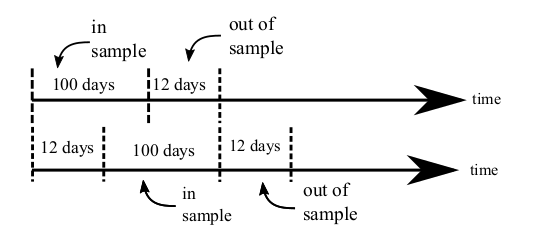
\includegraphics[width=3.5in,height=1.5in]{figures/backtesting_windows.png}}
	\label{backtetsing_window}
	\caption{Organisation of the rolling balancing and backtesting windows. \cite{notes}}
\end{figure}

More precisely, for day $t_i$ with $i$ in the following ranges, the backtest is in the corresponding balancing or evaluation phase:  

\begin{description}
	\item [$\bullet$ In sample (balance) window 1] - $t_i\:\forall\:i\:\in [0,99]$
	\item [$\bullet$ Out of sample (evaluation) window 1] - $t_i\:\forall\:i\:\in [100,111]$
	\item [$\bullet$ In sample(balance) window 2] - $t_i\:\forall\:i\:\in [12, 111]$
	\item [$\bullet$ Out of sample (evaluation) window 2] - $t_i\:\forall\:i\:\in [112, 121]$
\end{description}

This continues until the end of the 700 day dataset is reached. In total, the application balances 50 times, generates 50 new sets of weights, and evaluates these 50 times \textbf{for each target return}.

How this was achieved efficiently is outlined in the following section.

\subsection{Code}
\label{sec:implementation_code}


With a distinct focus on code readability, maintainability and efficiency, the backtesting frameworks, Quadratic Conjugate Method and other necessary tools to backtest the Markowitz optimised portfolio were written in C++ (which may be seen explicitly in the  \hyperref[sec:code]{code subsection} of the \hyperref[sec:appendix]{Appendix}, or in the \href{https://github.com/indipanesar96/markowitzportfoliooptimiser}{public repository}.).


The project code was split into five distinct project directories for the easy of maintenance and cleanliness. The directories and their contents are outlined briefly for context in the following sections.

\subsubsection{Utility}
\label{sec:utility}

The Utility contains the classes and structs \textit{VectorUtil, Matrix, RunConfig} and \textit{Results}. 
The first two housed small building-block-esque functions upon which the entirety of the application is based. As such, it was vital that these methods used to perform arithmetic operations on the rank 1 and 2 tensors were well tested and efficient. Creating these classes first greatly increased the speed and accuracy of development of the more complex classes that followed.
It was imperative that the arithmetic functions in \textit{VectorUtil} were as generic as possible. As a result, generic types were used throughout, though a condition was imposed in the typename signature that ensured the types being passed were numeric, as can be seen in the snippet below:


\begin{lstlisting}
// VectorUtil.h

template<typename T,
	typename = typename enable_if< is_arithmetic<T>::value, T> ::type>
vector<T> vectorLinearCombination(T aCoeff, vector<T> *a, T bCoeff, vector<T> *b) 
{
	int aSize = a->size();
	int bSize = b->size();
	if (aSize != bSize) {
		cout << "Vectors aren't the same size and so cannot be subtracted/added from/to one another." << endl;
		cout << "\t Sizes: " << aSize << " and " << bSize;
		exit(12);
	}
	vector<double> result = vector<double>(aSize);
	for (int i = 0; i < aSize; i++) {
		result[i] = aCoeff * a->at(i) + bCoeff* b->at(i);
}

return result;
\end{lstlisting}

Also seen in the above method is the helpful error message when it receives data incompatible with the operation, and an easily searchable error code for ease of debugging.


\textit{RunConfig}  and \textit{Results} are both C++ structs used to group pieces of information in a convenient manor. The former contained parameters that were pertinent to a particular run of the backtest. It was useful to run the application on small and medium sized subsets of the data for debugging purposes and so with each of these came a set of parameters (in/out of sample window lengths, for example) that were specific to the dataset in question. It became cleaner and more convenient to group these parameters together into one object (a \textit{RunConfig} struct) and pass this to \textit{Portfolio::backtest()}.  
The same philosophy was behind the use of the \textit{Results} struct as a return type from the aforementioned portfolio method as a way to group multiple result outputs together, instead of passing each object by reference or pointer individually. 

I found this line of reasoning to be especially pertinent with method signatures since their readability contributes massively to the readability of the application as a whole.  


\subsubsection{Repository}
\label{sec:repository}

Repository houses the classes and methods used to load data in from the comma separated value files. The functionality here was mostly provided with few other editions required.


\subsubsection{Estimator}
\label{sec:parameter_estimation}

This directory holds the \textit{ParamaterEstimator} class and its header, a prime example for the use case of a singleton object design pattern. The class holds public static methods that calculate various parameters such as the means, covariances and standard deviations of the aforementioned vector and self-made Matrix objects passed to it. It maintains no state and has no attributes; testament to the functional approach to programming commonly used when encoding mathematical functions.

\subsubsection{Optimiser}
\label{sec:portfolio_optimiser}

The \textit{PortfolioOptimiser} class and header are held in this directory and are where the Quadratic Conjugate Method is implemented. It was necessary for this class to maintain a state, having attributes on it that would be required across multiple of its methods. These attributes consisted of constant parameters from the \textit{RunConfig} of the current simulation, such as the initial values for the Lagrange Multipliers $\lambda$ and $\mu$ and the tolerance to which we declare the optimisation method as having converged. 

In addition, a getter and setter are employed to set the target return for the optimiser, $\overline{r_p}$ as the same instance of the \textit{PortfolioOptimiser} is used to solve for all different target returns.




\subsubsection{Backtest}
\label{sec:backtestcode}

The Backtest directory is where the \textit{Portfolio} class, header and \textit{main.cpp} were situated. The \textit{main.cpp} acted as the entry point into the application; where the \textit{RunConfigs} were initialised and sent to the aforementioned \textit{Portfolio::backtest()} method.

A matrix containing all returns data required for the simulation (a matrix of 700 rows by 83 columns in its entirety), was spliced with days acting to index the matrix; their values corresponding to the appropriate balancing and evaluating windows as described above.

For eahc window, the balancing window's matrix (in sample) of returns is passed by pointer to \textit{PortfolioOptimiser::calculateWeights()} which in turn calls a series of its own helper functions to return the weights. 

Once received \textit{Portfolio::checkWeights()} is called to ensure the sum of the weights is to within a predefined tolerance of unity (tolerance defined in \textit{RunConfig}). 

The weights are then passed with the test window's matrix (out of sample) to \textit{Portfolio::evaluate()} to evauluate the return of the portfolio over the out of sample window. The same weights are also passed with the in sample matrix of returns, generating the in sample returns ensuring the target return $\overline{r_p}$ is indeed achieved in sample. This also acts as a useful comparison to the out of sample portfolio returns achieved.

We now move to the discussion of the calculation of the weights themselves as the solution to Equation (\ref{matrix_solved}) by the Quadratic Conjugate Method.



\subsection{Quadratic Conjugate Method}
\label{sec:qcm}


Recall that the Markowitz Portfolio Choice Problem was reduced to a matrix equation of the form $Ax = b$ and that the Quadratic Conjugate Method solves this for vector $x$ numerically, with $x$ defined as:


\begin{equation}
x=
\begin{bmatrix}
\textbf{w}\\
\lambda \\
\mu
\end{bmatrix}
\end{equation}

An initialisation of $x_0$ is required for the method and so the weights \textbf{w} are chosen such that the initial portfolio is equally weighted (with a portfolio of $n = 83$ assets this is equivocates to setting all $w_i \approx 0.01205$). Inital values for the Lagrange Multipliers $\lambda$ and $\mu$ are set to 0.5 each though it was discovered that the initialisation of the two multipliers has little to no effect on the subsequent optimisation results.

A value of $\epsilon$ is required as our tolerance limit whereby convergence of the algorithm is defined when the length of the error term $s_{k+1}$ squared is less than $\epsilon$. This value is passed through to the private \textit{PortfolioOptimise::conjugateGradientMethod()} from the $RunConfig$ and a suitable value was found to be $10^{-6}$.

Though it must be noted that varying $\epsilon$ by a factor of $10^2$ smaller or larger seemed to have no effect on the rate of convergence. After some further investigation it was found that for the numbers typical to this context, the product $s_{k}'s_{k}$ jumps discontinuously from around $10^{-3}$ to $10^{-10}$. More generally, convergence has been proven to occur in fewer than iterations than the number of rows in matrix $A$ \cite{qcm_convergence}. This implies convergence is guaranteed in fewer than $n+2$ iterations, 85, in this dataset.

\newpage 


\begin{algorithm}
	\caption{Quadratic Conjugate Method} 
	
	Initialization: $k=0, s_0 \equiv b - Ax_0, p_0 \equiv s_0$;
	
	\begin{algorithmic}[1]
		\While {$s_{k}'s_{k} > \epsilon$}
		\State $\alpha_k = \frac{s_{k}'s_{k}}{p_{k}'Ap_{k}}$
		\State $x_{k+1} = x_{k} + 	\alpha_kp_{k}$
		\State $s_{k+1} = s_{k} - 	\alpha_kAp_{k}$
		\If{$s_{k+1}'s_{k+1} < \epsilon$}
		\State exit
		\EndIf
		\State $\beta_k = \frac{s_{k+1}'s_{k+1}}{s_{k}'s_{k}}$
		\State $p_{k+1} = s_{k+1} - 	\beta_kp_{k}$
		\State $k+=1$
		\EndWhile
	\end{algorithmic} 
\end{algorithm}


All variables apart from the result, $x_{k+1}$ are discarded when the thread leaves the scope of the loop as they are no longer required. Finally, the weights $w_{i}$ are retrieved from the first $n$ elements of $x_{k+1}$. 













\section{Results \& Discussion}
\label{sec:results}

Since this is an exercise in implementing a numerical optimisation method to financial data, the results of the application are judged by their adherance to the constraints imposed by the theory in \hyperref[theory]{section two}.

More specifically, the validity application will, in part, be measured by its ability to generate weights that form a portfolio yielding the target return specified.



\subsection{Accuracy}


\begin{figure}[H]
	\centerline{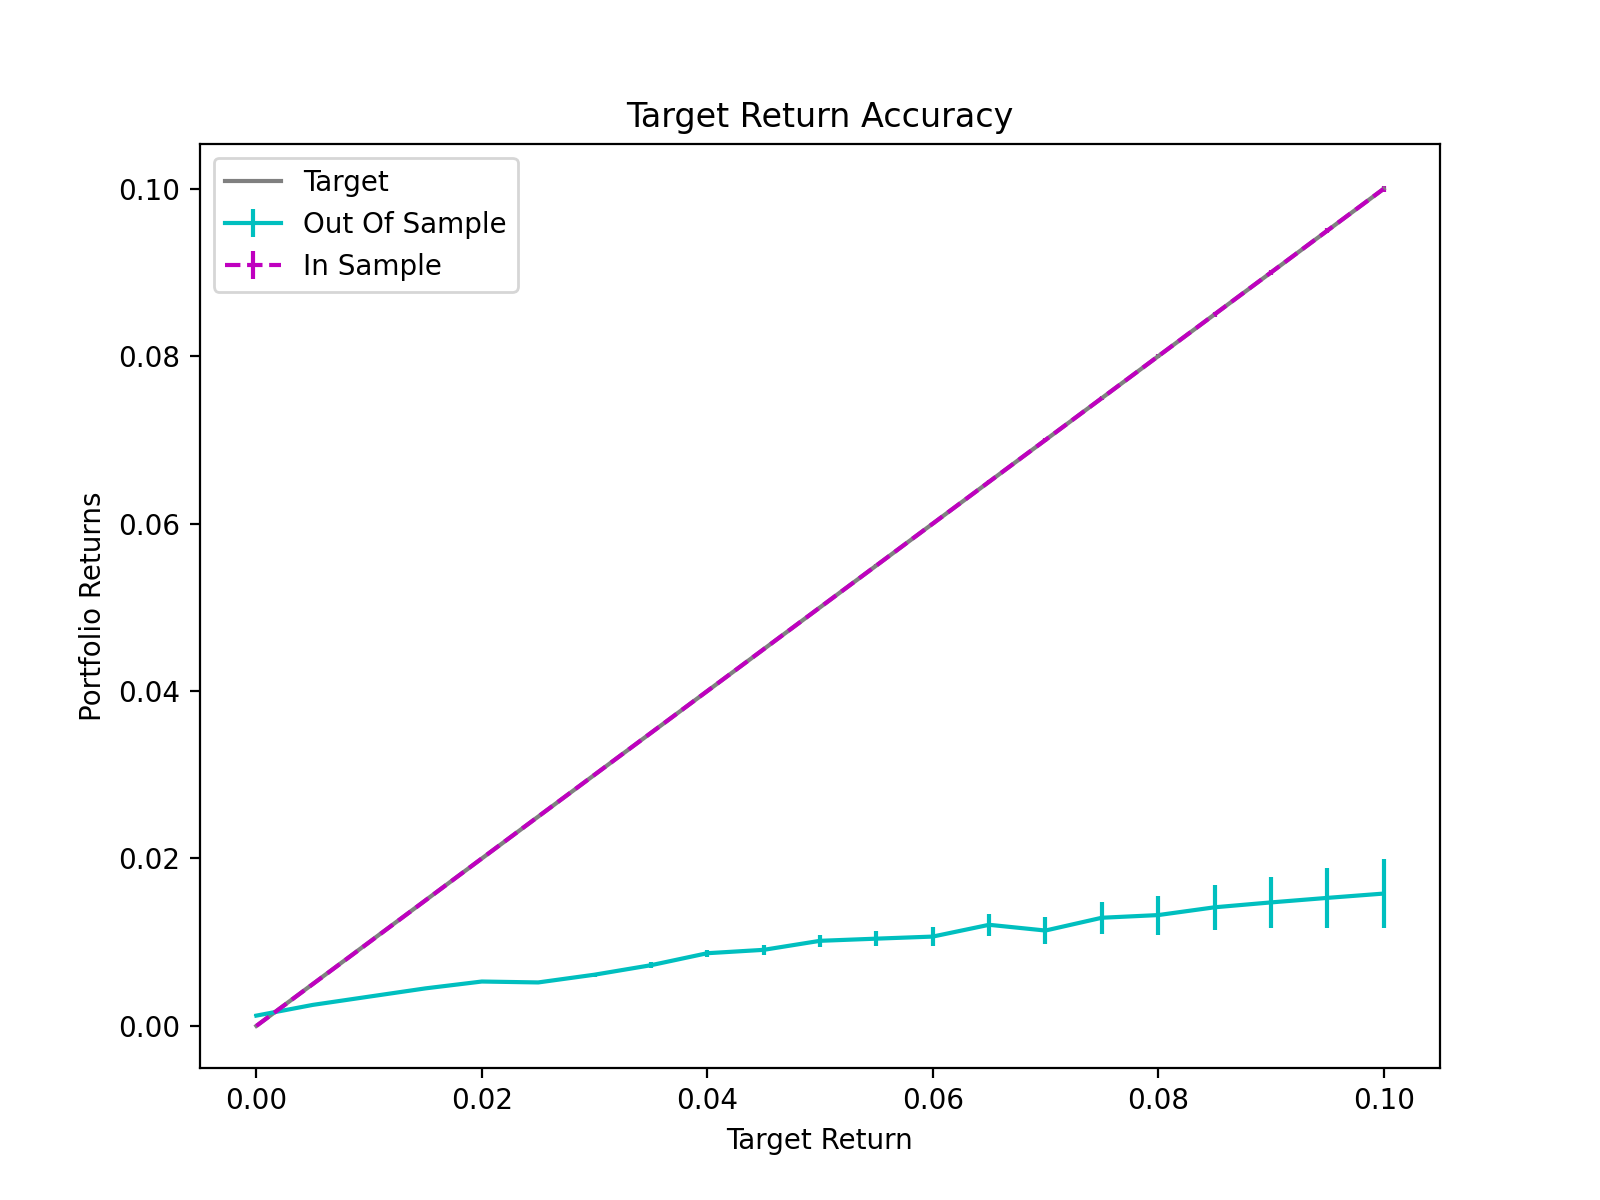
\includegraphics[width=3.5in,height=2.5in]{figures/oos_accuracy.png}}
	\label{oos_accuracy}
	\caption{A plot of the efficient frontier as generated by the application.}
\end{figure}



\subsection{Performance}

Since C++ was chosen as the language, the application's performance must be mentioned. Running the backtest across the full dataset of 700 days and $n=83$ assets a total of 20 times, the mean and standard error were calculated yielding a commendable took $14598.6 \pm 10.5\;ms$. EDIT THIS WITH NEW TIMES






BASICALLY TABLE THAT ALREADY GETS PRINTED OUT

TIME TAKEN TO RUN THE SCRIPT

EXPLAIN WHY STANDARD DEVS GETHIGHER AS RETURNS GET HIGHER - BECASUE WE CANT SEE IT IN THE DATA 9SINCE EXCESSIVELY LARGE RETURNS ARE LESS COMMON) -> MORE NOISE AND ERATICISM IN WEIGHTS PRODUCTION 

METHOD TENDS TO A LIMIT WHERE IT CANT PROCURE MORE RETURN SIMPLY BECAUE PORT RETURN IS WEIGHTS . RETURNS SO PORT RETURN IS LIMITED TO AT BEST, THE SAME RETURN AS THE BEST ASSET SEEN IN THE MARKET. (NO SHORT SELLING) - MAKE UP A SCENARIO WHERE WE SEE IT SHORT SELL A STOCK WITH A NEGATIVE RETURN --> METHOD WORKS


\section{Conclusions}
\label{sec:concs}


DECENT WAY TO OPTIMISE GIVEN HOW FAST CONVERGENCE IS


you may like to fix their values at the beginning.

Notice that you should not get (very) different results for different initialization values.

At the end of the day, this is a method that gives you the solution of a linear system!




\begin{thebibliography}{}
\label{sec:thebibliography}
	\bibitem{ef_medium} Medium. 2020. Fábio Neves. [ONLINE] Available at: https://towardsdatascience.com/python-markowitz-optimization-b5e1623060f5. [Accessed 8 June 2020].
	\bibitem{capm} Black, Fischer., Michael C. Jensen, and Myron Scholes (1972). The Capital Asset Pricing Model: Some Empirical Tests, pp. 79–121 in M. Jensen ed., Studies in the Theory of Capital Markets. New York: Praeger Publishers.
	\bibitem{mpt} Markowitz, H.M. (March 1952). "Portfolio Selection". The Journal of Finance. 7 (1): 77–91. doi:10.2307/2975974. JSTOR 2975974.
	\bibitem{notes} Parpas, P. "Computational Finance with C++, Numerical Methods for Optimization Models" pp. 27-37, Imperial College London
	\bibitem{qcm_convergence} Saad, Yousef (2003). Iterative methods for sparse linear systems (2nd ed.). Philadelphia, Pa.: Society for Industrial and Applied Mathematics. pp. 195. ISBN 978-0-89871-534-7.
	
	
	
\end{thebibliography} 



\section{Appendix} 
\label{sec:appendix}

\subsection{Additional Figures} 
\label{sec:add_figs}


\begin{center}
\begin{table}[H]
\begin{tabular}{|c c|} 
\hline
Run & Time Taken [ms]  \\ [0.5ex] 
\hline\hline
1 & 14760 \\
\hline
2 & 14519 \\
\hline
3 & 14557 \\
\hline
4 & 14569 \\
\hline
5 & 14551 \\
\hline
6 & 14575 \\
\hline
7 & 14593 \\
\hline
8 & 14601 \\
\hline
9 & 14598 \\
\hline
10 & 14594 \\
\hline
11 & 14588 \\
\hline
12 & 14620 \\
\hline
13 & 14582 \\
\hline
14 & 14602 \\
\hline
15 & 14591 \\
\hline
16 & 14600 \\
\hline
17 & 14609 \\
\hline
18 & 14607 \\
\hline
19 & 14610 \\
\hline
20 & 14646 \\ [1ex] 
\hline
\end{tabular}
\caption{The time taken for full runs of the backtesting application over all 83 assets and 700 days. \textbf{Mean} $\pm$ \textbf{ standard error: } $14598.6 \pm 10.5\;ms$}
\end{table}
\end{center}

\subsection{Code} 
\label{sec:code}




\end{document}